\chapter{Optimierungsstudie für die Alternativmethode}
%
\begin{figure}[h!]
  \subcaptionbox{\label{fig:acc0}}{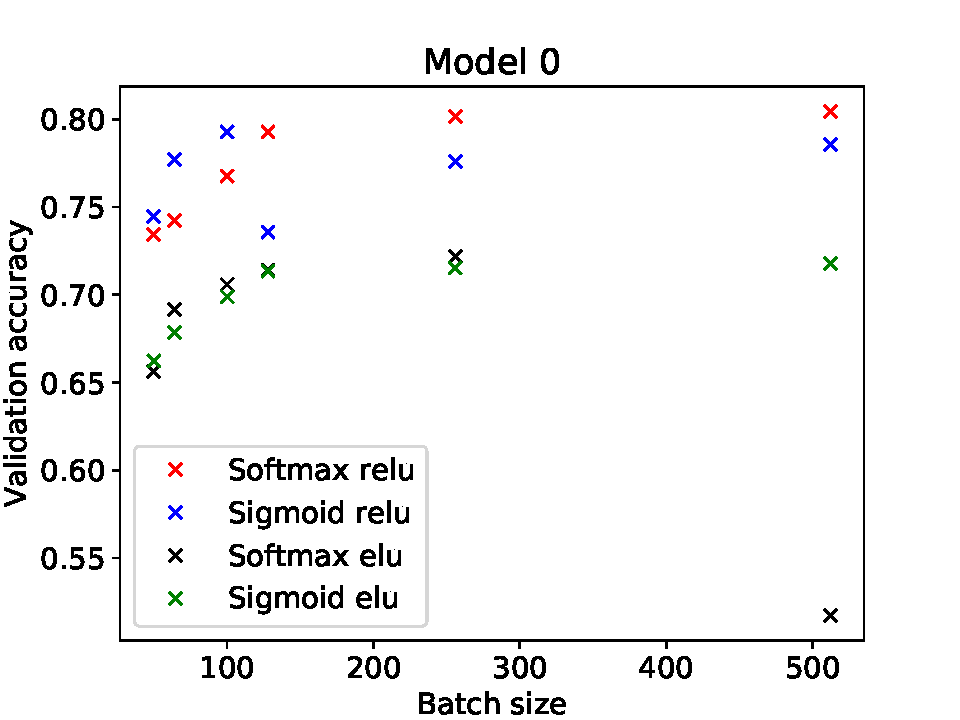
\includegraphics[width=0.3\linewidth]{Plots/Modelvalacc0.pdf}}
  \subcaptionbox{\label{fig:acc1}}{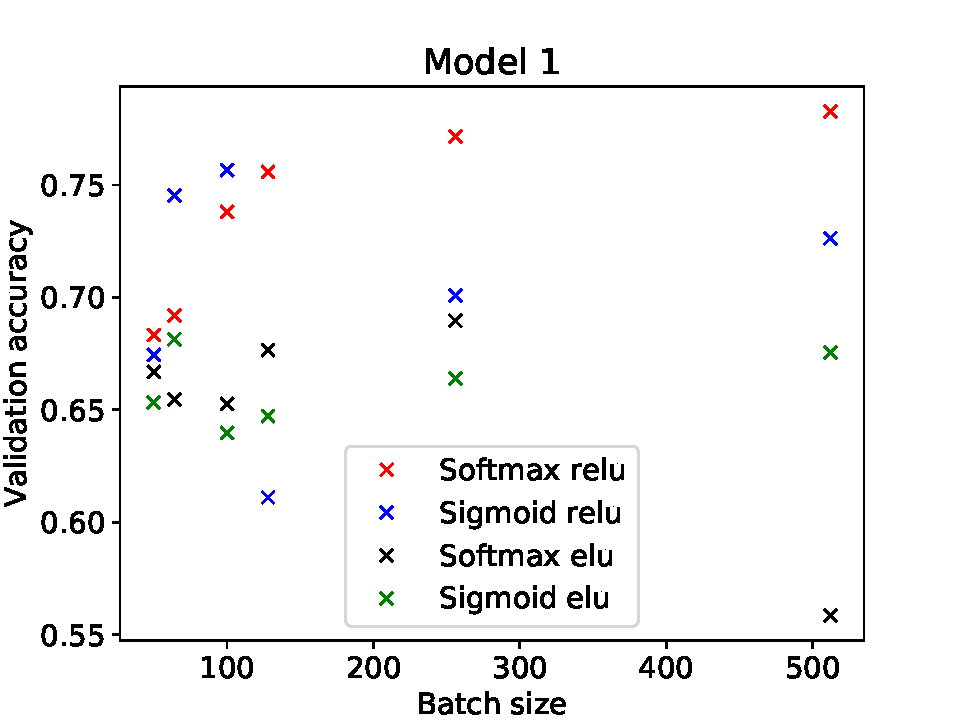
\includegraphics[width=0.3\linewidth]{Plots/Modelvalacc1.pdf}}
  \subcaptionbox{\label{fig:acc3}}{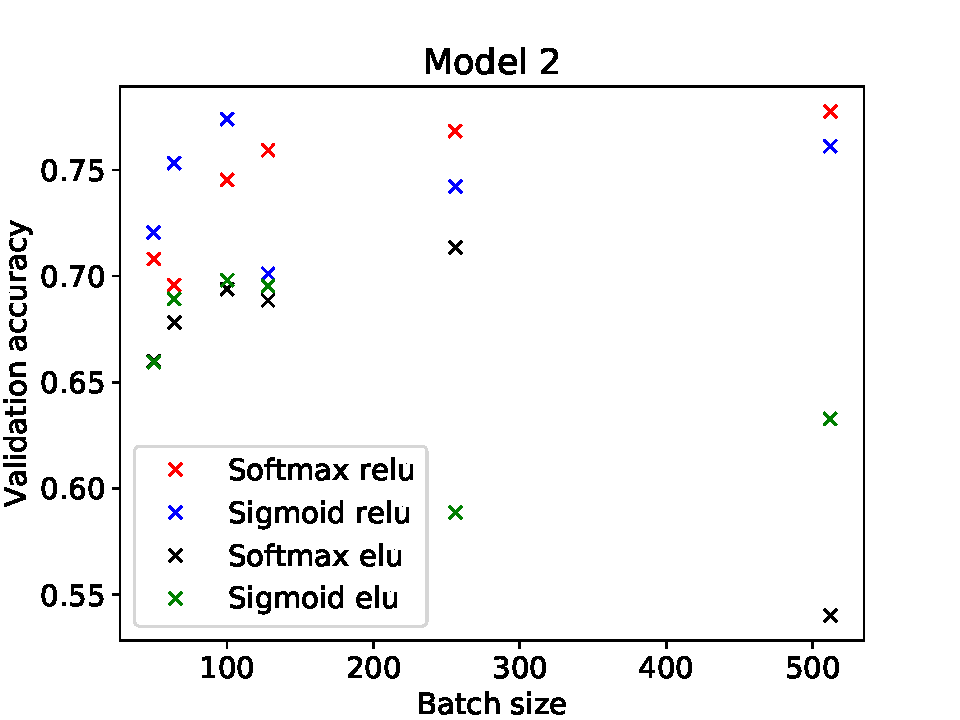
\includegraphics[width=0.3\linewidth]{Plots/Modelvalacc2.pdf}}
  \subcaptionbox{\label{fig:acc4}}{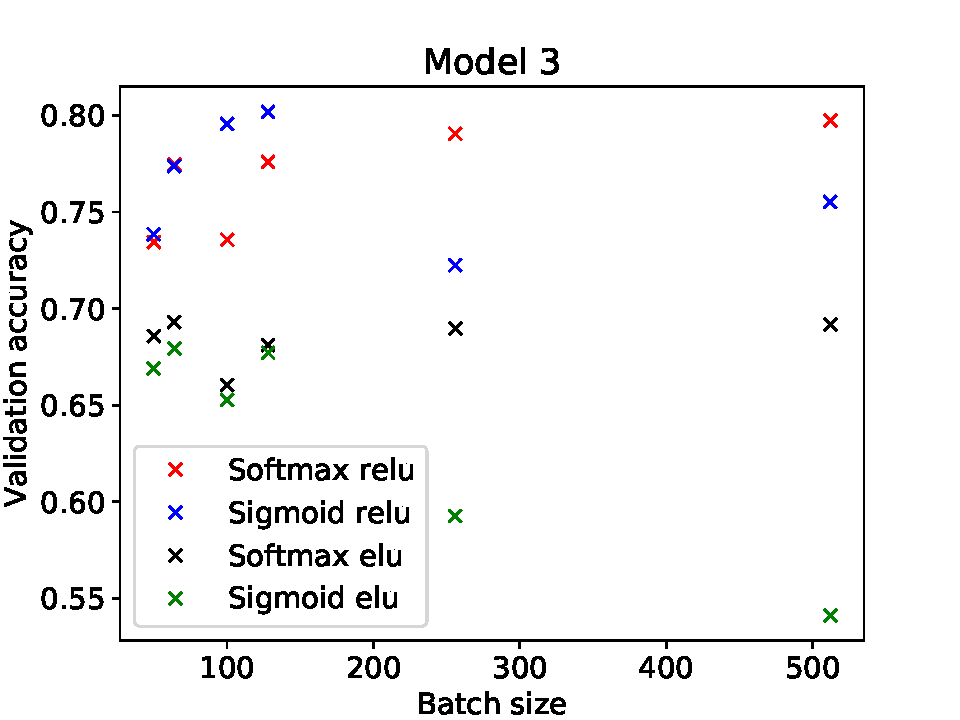
\includegraphics[width=0.3\linewidth]{Plots/Modelvalacc3.pdf}}
  \hspace{20pt}
  \subcaptionbox{\label{fig:acc5}}{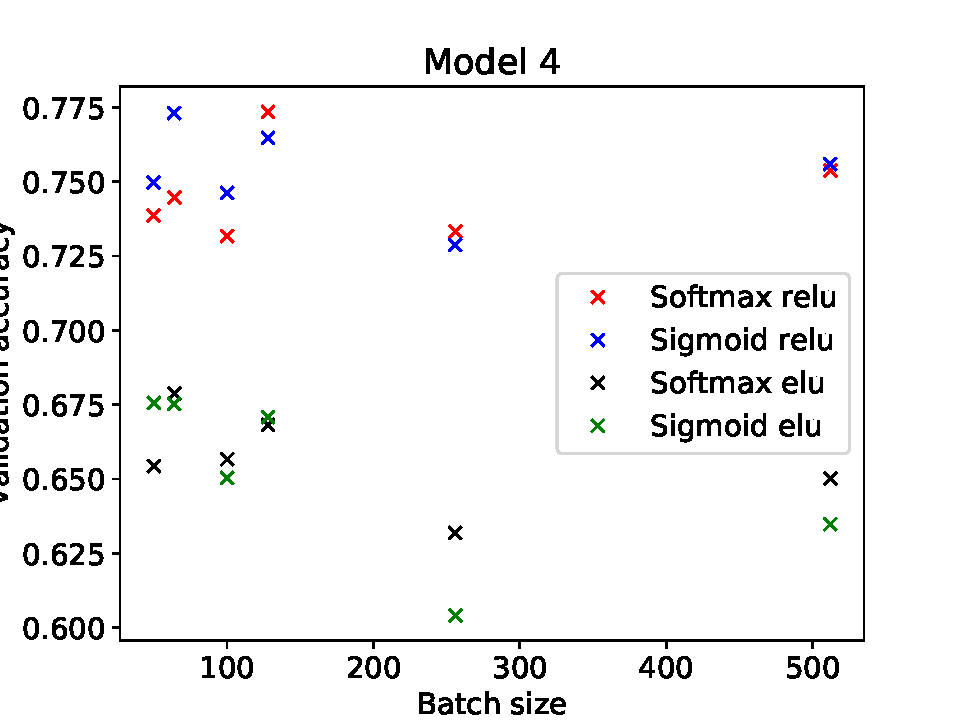
\includegraphics[width=0.3\linewidth]{Plots/Modelvalacc4.pdf}}
  \renewcommand{\baselinestretch}{1.0}
  \caption{Erreichte Genauigkeiten für die fünf Grundstrukturen der Alternativmethode. Die Genauigkeit ist in Abhängigkeit der \textit{batch size} für verschiedene Aktivierungsfunktionen dargestellt.}
  \renewcommand{\baselinestretch}{1.5}
  \label{fig:accs}
\end{figure}
%
%
\begin{table}
  \centering%
  \begin{tabular}{l
                  c
                  c}
      \toprule
      {}    & Anzahl der Dichtelagen + Filter     & Struktur der Dropout Lagen      \\
      \midrule
      Modell 0    & (1024, 512, 128, 64, 32)  & (0.5, 0.4, 0.4, 0.3, 0.2) \\
      Modell 1    & (1024, 512, 256, 128, 64, 32, 16)  & (0.5, 0.4, 0.4, 0.4, 0.2, 0.2, 0.1) \\
      Modell 2    & (512, 256, 128, 64, 32, 16)  & (0.4, 0.4, 0.3, 0.3, 0.2, 0.1) \\
      Modell 3    & (1024, 256, 64, 16)  & (0.6, 0.4, 0.2, 0.1) \\
      Modell 4    & (512, 128, 32)  & (0.5, 0.3, 0.1) \\
      \bottomrule
  \end{tabular}
  \caption{Getestete Grundstrukturen für die Netzarchitekturen der alternativen Methode.}
  \label{tab:grid}
\end{table}
%
%
\begin{figure}[h!]
  \subcaptionbox*{}{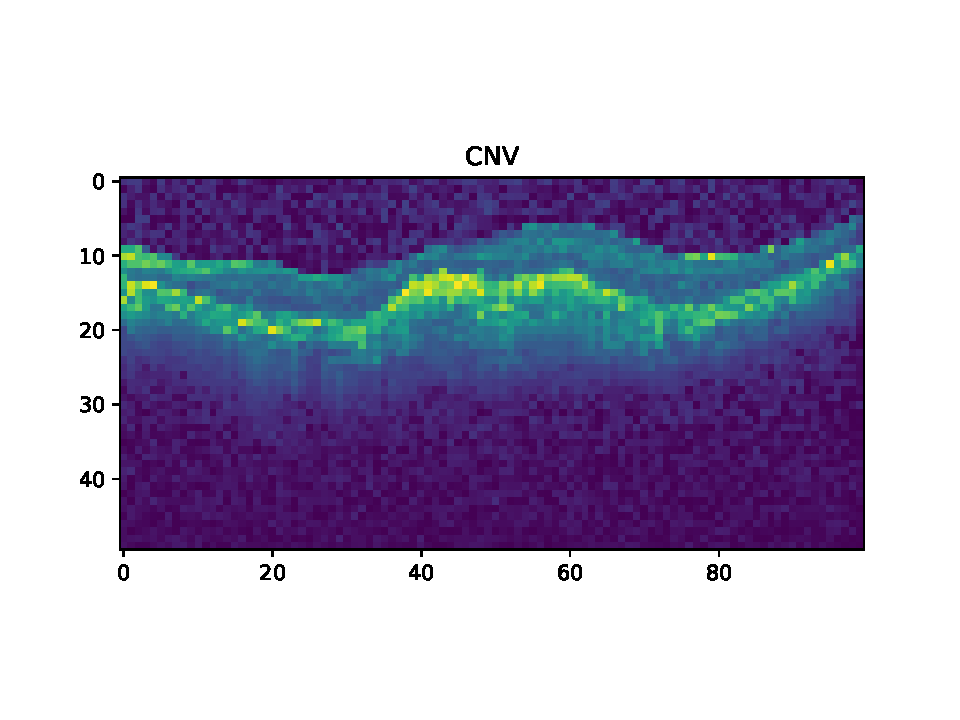
\includegraphics[width=0.3\linewidth]{Plots/Alternative_Beispiele/imageCNVscan.pdf}}
  \subcaptionbox*{}{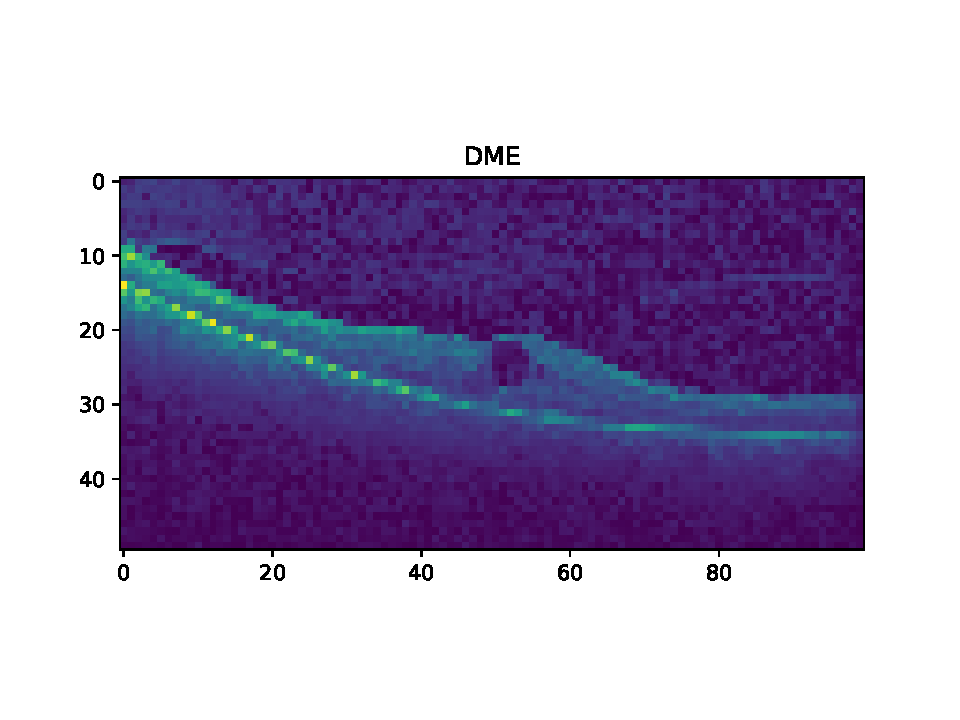
\includegraphics[width=0.3\linewidth]{Plots/Alternative_Beispiele/imageDMEscan.pdf}}
  \subcaptionbox*{}{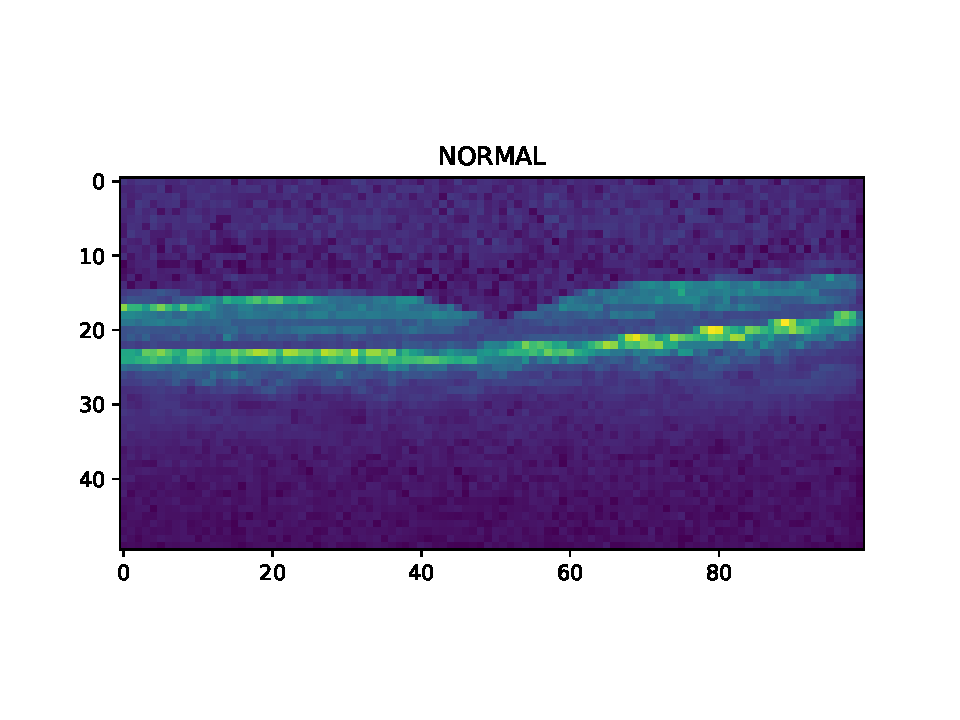
\includegraphics[width=0.3\linewidth]{Plots/Alternative_Beispiele/imageNORMALscan.pdf}}
  \subcaptionbox*{}{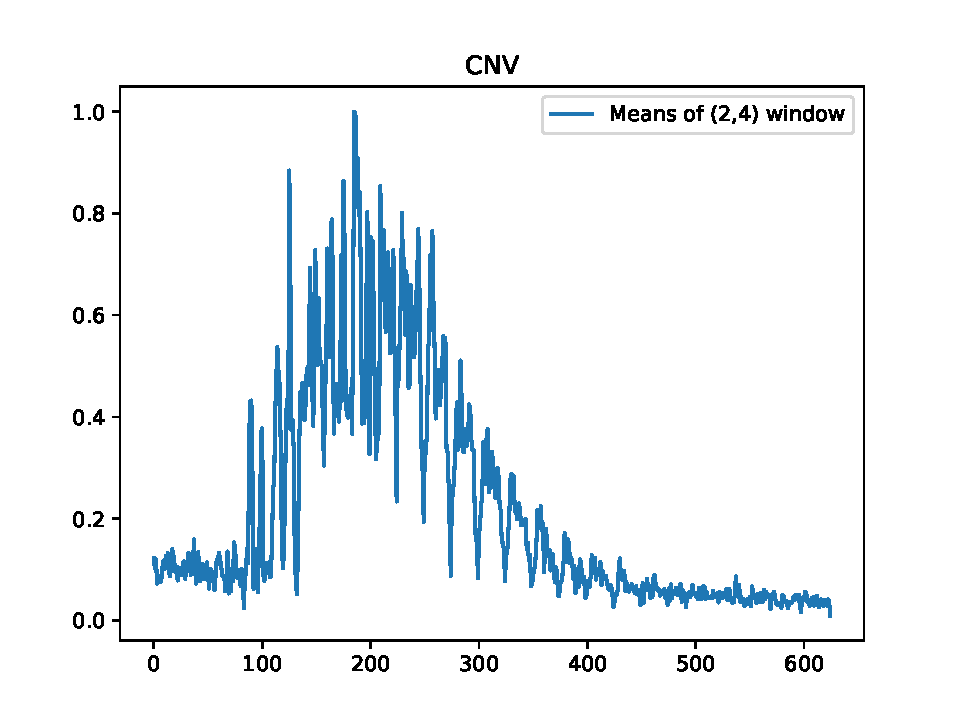
\includegraphics[width=0.3\linewidth]{Plots/Alternative_Beispiele/imageCNVmeans.pdf}}
  \subcaptionbox*{}{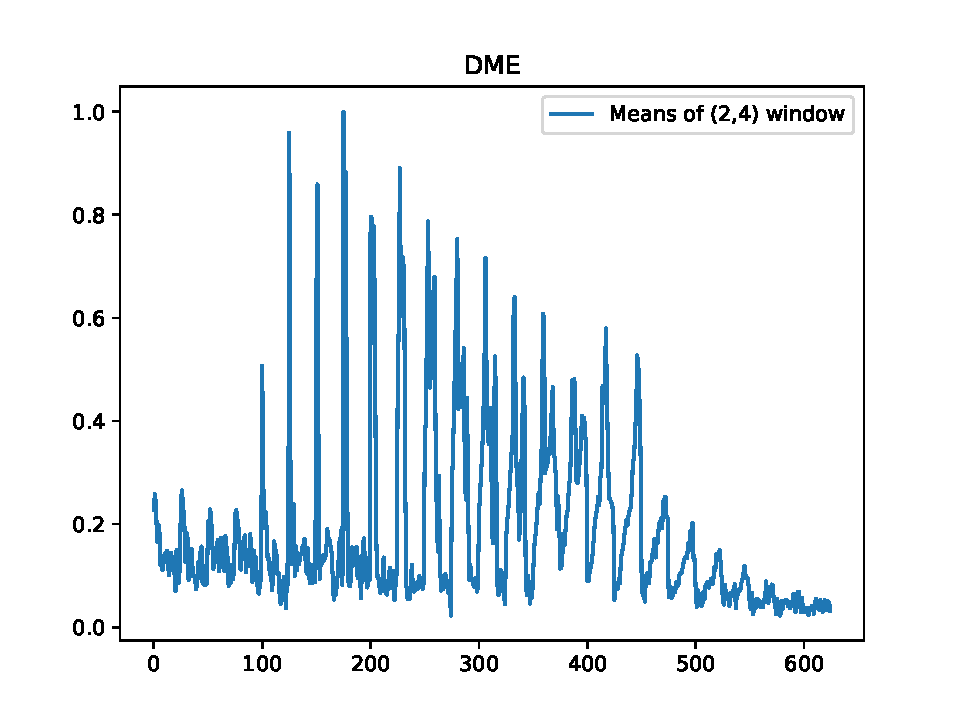
\includegraphics[width=0.3\linewidth]{Plots/Alternative_Beispiele/imageDMEmeans.pdf}}
  \subcaptionbox*{}{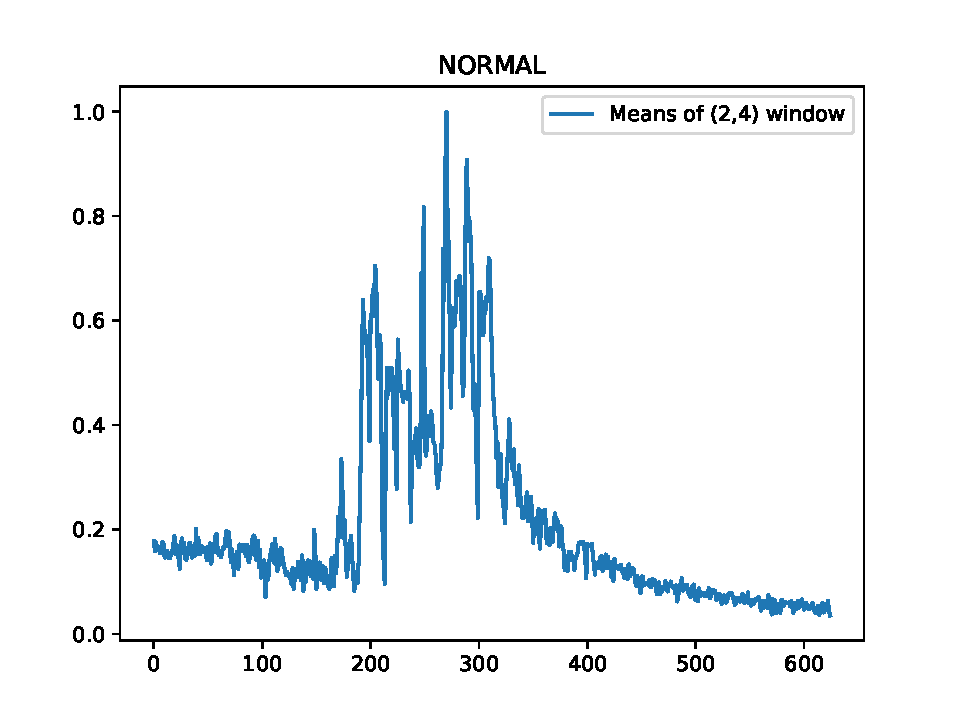
\includegraphics[width=0.3\linewidth]{Plots/Alternative_Beispiele/imageNORMALmeans.pdf}}
  \caption{Beispielbilder der anderen drei Klassen für die Skalierung der Bilder und die Bestimmung der Mittelwerte durch Abrastern im Rahmen der Alternativmethode.}
\end{figure}
%
